\section{Introdução}\label{introduuxe7uxe3o}

\begin{frame}{Sobre Mim}

\begin{itemize}
\itemsep1pt\parskip0pt\parsep0pt
\item
  Graduando em Ciência da Computação pelo IFCE.
\item
  7 anos de experiência com Linux.
\item
  Organizador do COMSOLiD a 6 anos.
\end{itemize}

\end{frame}

\begin{frame}{Introdução}

\begin{figure}
    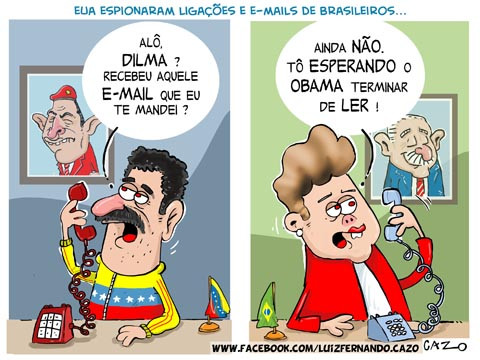
\includegraphics[scale=0.5]{img/Espionagem-por-Cazo.jpg}
    \caption{Nicolás Maduro e Dilma Rousseff}
\end{figure}

\end{frame}

\begin{frame}

\slidetitle{SSL} \slidesubtitle{Secure Socket Layer}

\end{frame}

\section{Acesso seguro através da
internet}\label{acesso-seguro-atravuxe9s-da-internet}

\begin{frame}{Acesso seguro através da internet}

Para acessar a internet com segurança usamos o protocolo SSL junto com o
HTTP.

\begin{figure}
    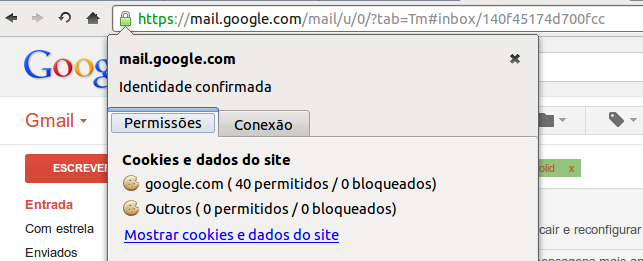
\includegraphics[scale=0.4]{img/gmail-ssl.png}
    \caption{SSL do Gmail}
\end{figure}

\end{frame}

\begin{frame}{Acesso seguro através da internet}

SSL é uma nova camada de protocolo que opera em cima do protocolo TCP.

Permite ambas as máquina, cliente e servidor, estabelecer uma conexão
criptografada.

\end{frame}

\begin{frame}{Acesso seguro através da internet}

Entretanto isso é uma especificação, ou seja, alguém tem que
implementar. Algumas empresas que o implementam:

\begin{itemize}
\itemsep1pt\parskip0pt\parsep0pt
\item
  OpenSSL (\href{openssl.org}{http://www.openssl.org/}) - Implementação
  livre e gratuita do SSL.
\item
  Apache-SSL (\href{apache-ssl.org}{http://www.apache-ssl.org/}) - um
  servidor web seguro, baseado no OpenSSL.
\item
  SSLeay (\url{ftp://ftp.uni-mainz.de/pub/internet/security/ssl/SSL/}) -
  uma implementação gratuita do Netscape's Secure Socket Layer.
\item
  Planet SSL
  (\url{http://www.rsasecurity.com/standards/ssl/developers.html}) -
  provê SSL para programas em C e Java.
\end{itemize}

\end{frame}

\begin{frame}[fragile]{Acesso seguro através da internet}

Exemplo de mesma implementação para problemas diferentes:

multiplicação de 2 números:

\begin{verbatim}
2 * 3
\end{verbatim}

ou

\begin{verbatim}
2 + 2 + 2
\end{verbatim}

\end{frame}

\begin{frame}

\slidetitle{Software Livre é seguro?}

\end{frame}

\begin{frame}{Software Livre é seguro?}

\begin{figure}
    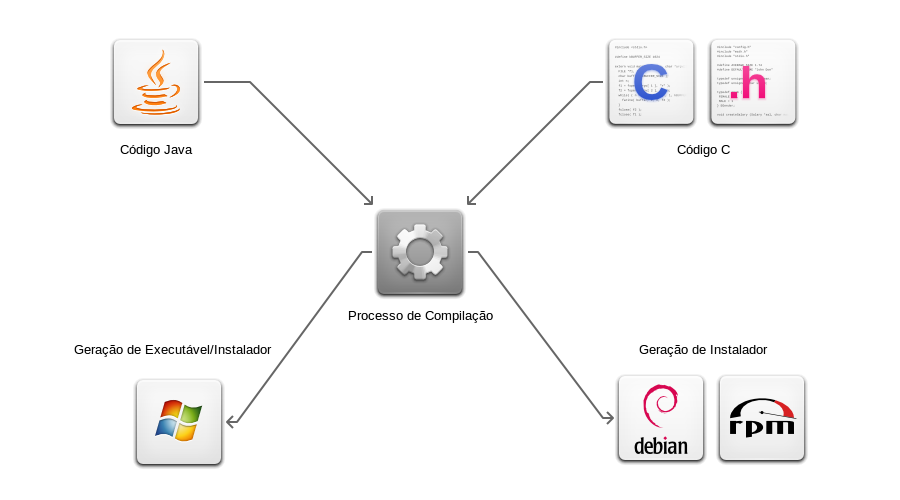
\includegraphics[scale=0.35]{img/codigos-compilados.png}
    \caption{Códigos Compilados}
\end{figure}

\end{frame}

\begin{frame}{Software Livre é seguro?}

\begin{figure}
    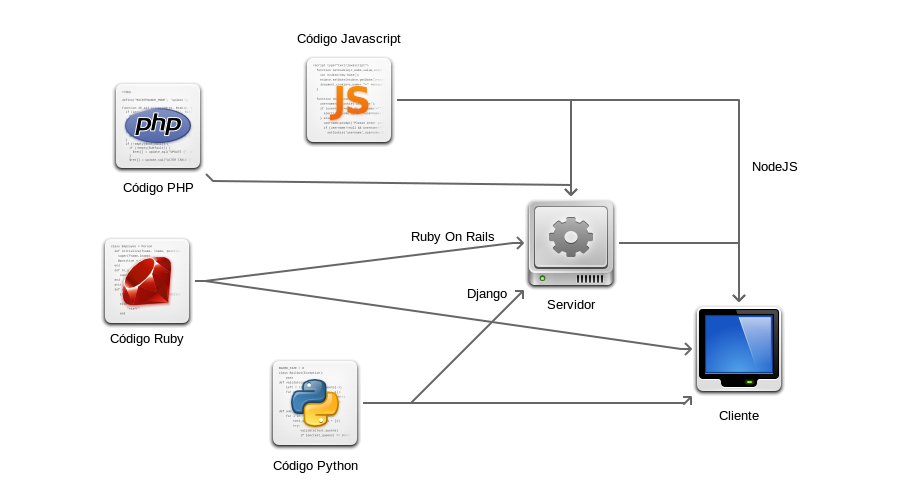
\includegraphics[scale=0.36]{img/codigos-interpretados.png}
    \caption{Códigos Interpretados}
\end{figure}

\end{frame}

\begin{frame}

\slidetitle{O quão é seguro uma criptografia usando SSL?}

\end{frame}

\begin{frame}

\slidesubtitle{Levaria um tempo significativamente maior que a idade do universo para quebrar uma chave de 128-bits.}

Estima-se um pouco mais de 13 bilhões de anos.

Fonte: \url{http://www.inet2000.com/public/encryption.htm}

\url{http://www.digicert.com/TimeTravel/math.htm}

\end{frame}

\begin{frame}

\slidetitle{Hackers e Crackers}

\end{frame}

\section{Hackers e Crackers}\label{hackers-e-crackers}

\begin{frame}{Hackers e Crackers}

\textbf{Crackers} são pessoas que invadem computadores com propósitos
criminais ou ganho pessoal.

\bigskip

Enquanto \textbf{Hackers} podem ser especialistas em segurança
contratados por empresas, com o objetivo de encontrar possíveis
vulnerabilidades e saná-las.

\end{frame}

\subsection{Hackeando Google e Duck Duck
Go}\label{hackeando-google-e-duck-duck-go}

\begin{frame}[fragile]{Hackeando Google}

Hackear é uma coisa boa! Alguns sites permitem que isso seja feito de
forma a otimizar processos, como fazer uma \textbf{busca}. Vejamos um
exemplo com o Google quando fazemos a seguinte busca:

\begin{verbatim}
comsolid filetype:pdf
\end{verbatim}

Além de buscar a palavra \texttt{comsolid}, ele busca apenas arquivos
\texttt{pdf}.

\end{frame}

\begin{frame}[fragile]{Hackeando Google}

Ou ainda podemos fazer buscas em determinados sites somente. Basta fazer
uma busca na forma:

\begin{verbatim}
inkscape site:comsolid.org
\end{verbatim}

Essa busca pesquisa a palavra \texttt{inkscape} no site
\texttt{comsolid.org}

\end{frame}

\begin{frame}{Hackeando Duck Duck Go}

\textbf{Duck Duck Go} é um motor de busca preocupado com a pesquisa em
si e sua privacidade.

\url{https://duckduckgo.com/}

Possui parte de seu código livre, isso inclui plugins, add-ons, etc.
Página do github:

\url{https://github.com/duckduckgo/}

\end{frame}

\begin{frame}{Hackeando Duck Duck Go}

Duck Duck Go permite \emph{hacks} mais engenhosos. Vamos a eles:

\begin{itemize}
\itemsep1pt\parskip0pt\parsep0pt
\item
  !g comsolid - busca comsolid no google
\item
  expand http://va.mu/dIwg - mostra a URL original
\item
  ip address - mostra seu endereço IP
\item
  github sige - mostra repositórios do github
\item
  @comsolid - mostra usuário do Twitter
\item
  age of linus torvalds - diz a idade
\item
  define free software - define uma palavra ou frase
\item
  weather in fortaleza - mostra a previsão do tempo
\item
  daft punk soundcloud - busca músicas no soundcloud
\end{itemize}

\end{frame}

\begin{frame}{Hackeando Duck Duck Go}

Temos ainda o \url{http://duckduckhack.com/}

\begin{figure}
    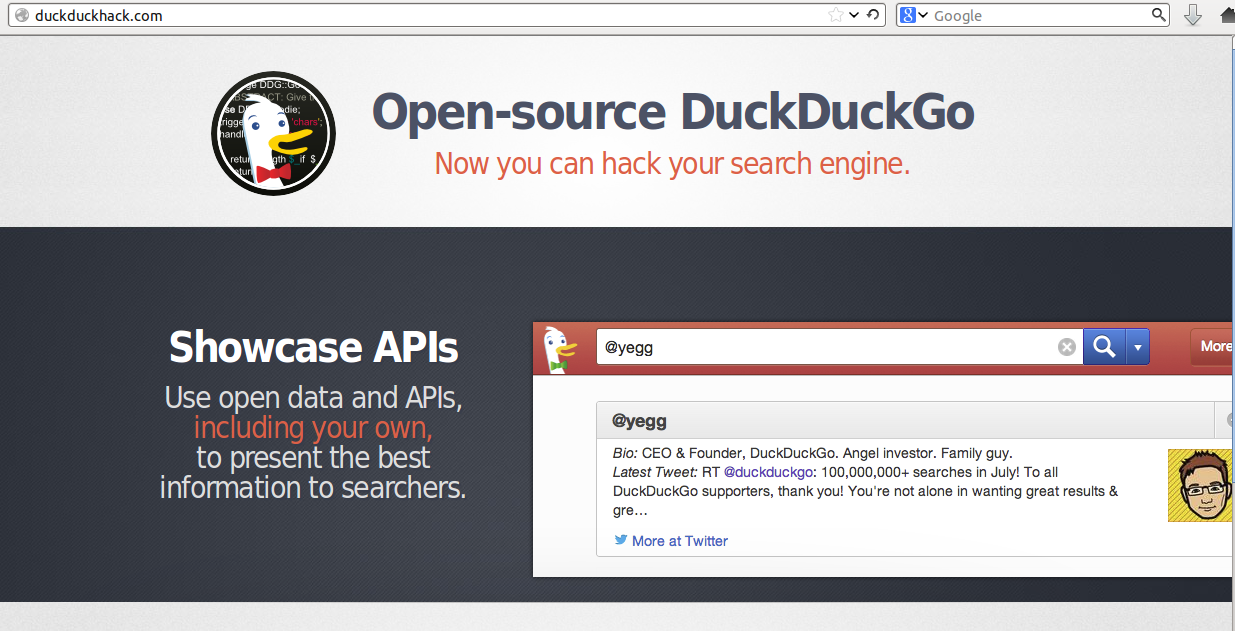
\includegraphics[scale=0.25]{img/duckduckhack.png}
    \caption{Duck Duck Hack}
\end{figure}

\end{frame}

\begin{frame}

\slidetitle{Técnicas para quebrar senhas}

\end{frame}

\subsection{Técnicas para quebrar
senhas}\label{tuxe9cnicas-para-quebrar-senhas}

\begin{frame}{Técnicas para quebrar senhas}

A técnica mais conhecida e natural é a força bruta, ou seja, tentar
todas as combinações possíveis até encontrar. Isso funciona até certo
ponto, quando a entrada é pequena.

Num artigo escrito por Dan Goodin no site \url{http://arstechnica.com}
em que descreve como Kevin Young, um pesquisador de segurança de senhas,
procedeu para descriptografar senhas vazadas pelo \textbf{Antisec} de
uma empresa chamada \textbf{Stratfor}.

\end{frame}

\begin{frame}{Técnicas para quebrar senhas}

Após quebrar 60\% das senhas usando listas de senhas disponíveis em:

\begin{itemize}
\itemsep1pt\parskip0pt\parsep0pt
\item
  Hashcat - \url{http://hashcat.net/oclhashcat-plus/}
\item
  John the Ripper - \url{http://www.openwall.com/john/}
\end{itemize}

Para os outros 40\% ele ficou ``sem palavras'', então onde encontrá-las?

Que tal Wikipedia, Youtube, Bíblia, Projeto Gutenberg?

\end{frame}

\begin{frame}{Técnicas para quebrar senhas}

Uma das senhas era ``crotalus atrox'', nome científico de uma cobra. Tal
senha foi quebrada graças a esta página da Wikipedia:
\url{https://en.wikipedia.org/wiki/Crotalus_atrox}

Em seguida outras senhas fortes por serem grandes foram encontradas
como:

\begin{itemize}
\itemsep1pt\parskip0pt\parsep0pt
\item
  ``from genesis to revelations'' (26)
\item
  ``I cant remember anything'' (24)
\item
  ``thereisnofatebutwhatwemake'' (26)
\item
  ``givemelibertyorgivemedeath'' (26)
\end{itemize}

\end{frame}

\subsection{Vazamento de senhas ao
Linkedin}\label{vazamento-de-senhas-ao-linkedin}

\begin{frame}{Vazamento de senhas ao Linkedin}

Em Junho de 2012 um usuário anônimo postou no site
\url{http://insidepro.com/} uma lista com 6.5 milhões de hashs únicos
referentes a senhas pedindo ajuda para recuperá-las.

Após quebrar muitas das senhas descobriu-se que se tratava de um banco
de senhas do site Linkedin. Essa descoberta foi possível pelo número de
senhas com a palavra \emph{linkedin}.

\end{frame}

\begin{frame}{Vazamento de senhas ao Linkedin}

Na lista existiam:

\begin{itemize}
\itemsep1pt\parskip0pt\parsep0pt
\item
  1 - linkedin (4408)
\item
  2 - link (2638)
\item
  3 - linked (2135)
\end{itemize}

Outras senhas encontradas:

\begin{itemize}
\itemsep1pt\parskip0pt\parsep0pt
\item
  8 - love (1018)
\item
  11 - password (856)
\item
  16 - abc (750)
\end{itemize}

Mais informações em:
\url{http://www.ma.rhul.ac.uk/static/techrep/2013/MA-2013-07.pdf}

\end{frame}

\subsection{Engenharia reversa em firmware
D-Link}\label{engenharia-reversa-em-firmware-d-link}

\begin{frame}{Engenharia reversa em firmware D-Link}

Todos sabemos que a D-Link é especializada em fazer roteadores, e eles
são um bom local para \emph{backdoors}. E isso foi exatamente que Craig
Heffner autor no blog \url{http://www.devttys0.com} encontrou.

Ele encontrou a partir de uma engenharia reversa no firmware de uma dos
roteadores.

\end{frame}

\begin{frame}{Engenharia reversa em firmware D-Link}

Após notar que certa função chamada \texttt{alpha\_auth\_check} soava
suspeita, ele foi saber o que exatamente ela fazia. Após um tempo ele
chegou no seguinte trecho de código:

\inputccodefile{ src/d-link.c }

\end{frame}

\begin{frame}{Engenharia reversa em firmware D-Link}

Baseado no código fonte das páginas HTML e outros detalhes é sensato
concluir que os seguintes modelos são afetados:

\begin{itemize}
\itemsep1pt\parskip0pt\parsep0pt
\item
  DIR-100
\item
  DIR-120
\item
  DI-624S
\item
  DI-524UP
\item
  DI-604S
\item
  DI-604UP
\item
  DI-604+
\item
  TM-G5240
\end{itemize}

\end{frame}

\begin{frame}{Engenharia reversa em firmware D-Link}

Quem quiser fazer um teste real existe um código em Python escrito pelo
próprio Craig e pode ser encontrado em:

\url{http://pastebin.com/vbiG42VD}

\inputpycodefile{ src/trecho-backdoor.py }

\end{frame}

\begin{frame}

\slidetitle{Ataque ao Kernel}

\end{frame}

\subsection{Ataque ao Kernel}\label{ataque-ao-kernel}

\begin{frame}{Ataque ao Kernel}

\url{http://linux.slashdot.org/story/13/10/09/1551240/the-linux-backdoor-attempt-of-2003}

Em 2003, houve uma tentativa de backdoor no Kernel do Linux.

\inputccodefile{ src/backdoor.c }

Bastava chamar a função \texttt{wait4} e você viraria \emph{root}.

\end{frame}

\begin{frame}{Ataque ao Kernel}

Comparemos os códigos original e o backdoor, e vejam se encontram a
diferença.

\inputccodefile{ src/original.c }

\inputccodefile{ src/backdoor.c }

\end{frame}

\section{Marco Civil da Internet no
Brasil}\label{marco-civil-da-internet-no-brasil}

\begin{frame}{Marco Civil da Internet no Brasil}

\textbf{O que é Marco Civil?}

É um projeto de Lei que visa estabelecer direitos e deveres na
utilização da Internet no Brasil. É a constituição da Internet no país.

\end{frame}

\begin{frame}{Quais são os direitos e deveres?}

\begin{itemize}
\itemsep1pt\parskip0pt\parsep0pt
\item
  \textbf{Neutralidade}: proíbe que provedores de internet discriminem
  certos serviços em detrimento de outros.
\item
  \textbf{Armazenamento de dados}: Operação de coleta de dados no Brasil
  deve respeitar a privacidade, proteção dos dados e sigilo das
  comunicações privadas.
\item
  \textbf{Retirada de conteúdo}: entidades que oferecem conteúdo e
  aplicações só serão responsabilizadas por danos gerados por terceiros
  se não acatarem ordem judicial exigindo a retirada dessas publicações.
\end{itemize}

\end{frame}

\begin{frame}{Quais são os direitos e deveres?}

\begin{itemize}
\itemsep1pt\parskip0pt\parsep0pt
\item
  \textbf{Fim do marketing dirigido}: as empresas de acesso não poderão
  ``espiar'' o conteúdo das informações trocadas pelos usuários na rede.
  Há interesse em fazer isso com fins comerciais, como para publicidade.
\item
  \textbf{Sigilo e privacidade}: Provedores de acesso à internet serão
  obrigados a guardar os registros das horas de acesso e do fim da
  conexão dos usuários pelo prazo de seis meses, mas isso deve ser feito
  em ambiente controlado.
\end{itemize}

Para mais detalhes:
\url{http://www.molon1313.com.br/marco-civil-da-internet/}

\end{frame}

\begin{frame}{Onde encontrar essa palestra?}

\begin{center}
Você pode baixar essa palestra e ainda outras em:

\bigskip

\large{\url{http://sige.comsolid.org/u/atilacamurca}}
\end{center}

\end{frame}

\begin{frame}

\slidetitle{Dúvidas?}

\end{frame}

\begin{frame}{Conecte-se}

\begin{center}
E-mail:\\
\texttt{camurca.home@gmail.com}

\medskip

Twitter:\\
\url{http://twitter.com/\#!/atilacamurca}

\medskip

Blog MAD3 Linux:\\
\url{http://www.mad3linux.org}

\medskip

COMSOLiD:\\
\url{http://comsolid.org/}\\
\url{http://twitter.com/\#!/comsolid}\\
\url{https://www.facebook.com/comsolid}

\medskip

Github:\\
\url{https://www.github.com/atilacamurca}
\end{center}

\end{frame}
